\documentclass[11pt,titlepage]{report}
\usepackage[a4paper]{geometry}
\usepackage{hyperref}
\usepackage{listings}
\usepackage{graphicx}
\begin{document}
\title{Story Evolution Tracker: Preliminary Report}
\author{Violet Avkhukova\\Student Number: 1573866\\Email: violetta.avkhukova@kcl.ac.uk\\Advanced Software Engineering\\King's College London\\\\\\Supervised by\\Dr. Odinaldo Rodrigues\\}
\maketitle

% Configurations:
\lstset{basicstyle=\ttfamily, breaklines=true}
\setlength{\parskip}{-0.5em}

\chapter{Introduction}
\section{Motivation}
\paragraph{}
The ways in which people read the news have evolved. With the rapid growth and accessibility of the Web, many news sources provide news stories online in addition to traditional newspapers \cite{alipes}. Online news reach more people than ever before, with thousands of unique users on websites such as Yahoo and Daily Mail each month \cite{digital_trends}. Not only has the Web shifted focus to online news, the way news is accessed online is shifting towards mobile devices. In a survey of 50 top news websites, 39 had more mobile users than desktop \cite{digital_trends}. Despite the mobile trend, only 10 out of 50 news websites had mobile visitors spend more time per visit \cite{state_of_news}.
\paragraph{}
The statistics suggest that mobile users do not like spending a lot of time digesting news on their devices. A viable solution to this is to condense news to a length that is deemed short enough to read in a small amount of time, while still receiving all the important details of the article, that is, creating a summary.
\paragraph{}
Not only has the Web provided many time-consuming articles to read, different sources may present the same news topic or event with different perspectives. To recieve all these differences of opinion, a lot of manual work would be required to find such articles. And finally, if a news story goes through updates and developments, the user would normally need to get notified by some source and then read the entire article, which they normally do not like to do.
\section{Aims and Objectives}
\paragraph{}
The goal of this project, called the Story Evolution Tracker (SET), is to address all these issues at hand. The following is a description of the requirements of the SET. The SET will track news stories and how they evolve over time. The user will specify a link to a news story from a pre-defined source and the system will begin tracking it. Any developments that are made will be added to the story's timeline and reported to the user. A \textit{signature} will be created for identification of the news topic, even if it changes over time. The signature will include a basic summary of all the events that happened since the beginning of tracking. The system will also learn about the user's interests and provide articles that he or she may like to read or track.
\paragraph{}
There are many things to consider in this project, such as what processes will go into generating signatures, whether to look at past articles for contextual background, how often to query for news story developments, how much of the original news articles to send to the user, and much more. 
\section{Report Structure}
\paragraph{}
The rest of this report is broken up into multiple chapters, each discussing different work that has gone into this project. Chapter 2 will discuss the background for the Story Evolution Tracker, including required technical background knowledge and past works done in fields similar to the requirements of this project. Chapter 3 will discuss system design, which includes technical requirements and a plan for development and methodologies. 
\chapter{Background}
\section{Technical Background}
\paragraph{}
The following concepts are required in the understanding of this project and will be involved in the implementation of the objectives. A brief description of each is presented. These concepts include HTML, HTTP, natural language processing, and machine learning. 
\subsection{HTML and HTTP}\label{html_http_section} 
\paragraph{}
Because of the nature of this project, some knowledge of HTML and the Hypertext Transfer Protocol (HTTP) is required. Web pages are represented by HTML code, which contains everything needed to render it in the browser. It is the standard markup language for the web, providing a structure of elements \cite{w3c_html}. Elements, such as the paragraph element, may contain useful content, like news story content. Div tags create containers of data or other elements that can be identified by an id or class name, which can also contain useful content. A browser builds a Document Object Model (DOM), an abstract representation of HTML structure that allows dynamic updates and queries of the structure \cite{practical_jquery}.
\paragraph{}
To get the HTML code from pages, HTTP will be used, the standard web protocol for transfer of data. Using the HTTP request method with the GET parameter, the content of the given URL is requested. The content is received as an HTTP response containing a response-body which holds the requested content \cite{RFC2616}. With use of HTTP, the contents of any web page can be accessed.
\subsection{Natural Language Processing}
\paragraph{}
Natural language processing (NLP) is defined as the study of natural language, using computer science aspects, to derive meaningful information from text. Some NLP difficulties lie in language ambiguity, word variety, and semantics, but sentences generally follow grammatical and syntactic rules \cite{nlp_java}. Processes involved in NLP include finding parts of a text, sentences, relationships between text, and classifying documents. 
\paragraph{}
In this system, the main NLP aspect utilized will be summarization for generating a topic signature. Sparck Jones defines summarization as a "reductive transformation ... through content condensation by selection and/or generalisation on what is important in the source" \cite{state_of_the_art}. Before summarization can take place, several text processes must take place, such as splitting the text into segments, normalizing words, and filtering out stopwords \cite{torres}. General summarization processes include taking a source text, interpreting it to create an internal representation, then transforming that into an internal summary representation, and finally transforming that into a text representation \cite{state_of_the_art}. This project will explore summarization techniques for generating signatures for an evolving news story topic.
\paragraph{}
One common algorithm for determining the importance of a word in a document or set of documents is the tf-idf (term frequency-inverse document frequency) algorithm. Words that occur too frequently, such as stop words, would occur many times in many documents, so their tf-idf values will tend to zero, i.e. not important. However, this depends on the corpus of documents that is used. Words that may be of actual importance could appear in each document, but its inverse document frequency can still tend to zero. Generally, this algorithm is simple to implement and gives good results \cite{torres}, so it could be used as a method of determining key words in a document.

\subsection{Machine Learning}
\paragraph{}
Machine learning is the process of using data to derive results that cannot be arrived at trivially. In general, algorithms are applied to an input to get some output. However, in the realm of machine learning, such algorithms may not exist and only an approximation can be achieved \cite{alpaydin}. Machine learning relies a lot on statistics and probability to achieve these approximations. One machine learning task is classification. Given an input, a classifier assigns a class, or label, based on some probabilistic knowledge. Therefore, the main goal is prediction: learning an association between two values.
\paragraph{}
For processing text, data is usually represented as a vector, which can hold word frequencies, weights, or other measures. It is simpler to do calculations on vector representations \cite{smola}. One known machine learning algorithm is the Naive Bayes' classifier algorithm. It is based on Bayes' Rule, which calculates the probability of event A, having observed event B \cite{alpaydin}. However, in some predictions, we may not have all probabilities available to use, such as the probability of event B, having observed event A \cite{smola}. In the Naive Bayes' algorithm, all inputs are assumed to be independent, ignoring all possible dependencies and correlations \cite{alpaydin}. The problem is reduced "from a multivariate problem to a group of univariate problems", and thus reducing the complexity \cite{alpaydin}. 
\paragraph{}
Another known machine learning algorithm is the k-Nearest Neighbour algorithm.  An object is classified according to its' k nearest neighbours, where k is some value set by the user. The k value is much smaller than the total number of objects present in the system \cite{alpaydin}. First the similarity of the object to other objects is computed using a similarity algorithm, such as cosine similarity or Euclidian distance \cite{torres}. The classification is then determined by the majority-winning class label in the surrounding k neighbours. This algorithm is considered one of the simplest machine learning algorithms and can be widely used in many applications, but is limited in some ways because it only focuses on a subset of the data when determining the classification \cite{nearest_neighbour}.
\section{Previous Work}
\paragraph{}
The following sections will describe work done by others in the fields of HTML extraction and parsing, text summarization, and learning and modeling user interests. 
\subsection{HTML Extraction and Parsing}
\paragraph{}
Because the nature of this project is to deal with HTML documents, the following analysis of previous works is appropriate. To get meaningful information from a web page, first its HTML code must be extracted and parsed. HTML extraction from a URL is trivial; using HTTP GET requests, as described in section \ref{html_http_section}, the contents of a web page can be collected. However, there have been numerous works done for parsing HTML code. 
\paragraph{}
The first work investigated is the WysiWyg Web Wrapper Factory (W4F) created by Sahuguet and Azavant \cite{w4f}. The main system is a web wrapper that converts HTML code to a data-structure representation for manipulation. They defined a three step process: retrieving the document using some retrieval rules, extracting data from it using some extraction rules, and finally exporting it using some mapping rules. Different granularities during the extraction step are possible, such as retrieving tables and lists but also information from within a tag. Retrieving the HTML document is done by the standard HTTP GET request. 
\paragraph{}
Next is the extraction step. They created an HTML Extraction Language (HEL) which contains extraction rules for a given type of document \cite{w4f}. To navigate the HTML structure, it is first parsed into a DOM tree to represent the hierarchy. Once built, the tree can be navigated using the document hierarchy or the flow of the document. An example of using document hierarchy is "html.head[0].title[0]", where the dot operator signifies going down a level \cite{w4f}. Using the flow of the document is similar, but using depth-first search for the requested element. The next step is to extract information from the elements that are found through DOM tree navigation. The nodes themselves are uninteresting; it is the data they contain that is important. By using regular expressions, data is found, matched, and returned from a node. Nested list structures are created to extract multiple pieces of information. The final system was presented as a toolkit with multiple wizards for each step of the process \cite{w4f}.
\paragraph{}
Although this system can perform the required task of parsing and extracting information from HTML code, it has some significant limitations. Firstly, the navigation of the DOM tree is dependent on the index of each type of element, i.e. where it is actually located in the tree. Therefore, it would be required to know exactly where the desired element is in the document. However, the structure of web pages can change and the element may no longer be at that location. Secondly, the use of regular expressions to extract element information can encounter some issues. The pattern required for each web page can change as well as the pattern for each kind of element. Regular expressions may also need to be changed if the layout of information changes in the element. 
\paragraph{}
The second work investigated is jQuery. jQuery is a well-known JavaScript library for extracting useful information from HTML \cite{jquery}. Created by John Resig, this library allows cross-browser compatability for DOM tree manipulation \cite{practical_jquery}. First, the DOM tree representation of the HTML is required. The browser builds this and jQuery can use it for data extraction. The main functionality is selecting DOM tree elements using CSS-style selectors. General syntax follows the pattern \lstinline|$(selector).action();| \cite{practical_jquery}. Consider the following HTML code: \lstinline|<div id="myDiv" class="allDivs">Hello World</div>|. This div can be selected by the following jQuery lines: \lstinline|$("#myDiv")| or \lstinline|$(".allDivs")|. The text "Hello World" can be extracted by appending \lstinline|.text()| to either line of code \cite{jquery_text}. In short, jQuery is used to get specific sections of an HTML document based on its element type, id, or class. 
\paragraph{}
Because of how simple, minimal, and readable jQuery is, it became widely popular and important in the web development community \cite{practical_jquery}. The complexity of retrieving information from a web page was greatly reduced. There are many advantages of using this approach. Firstly, knowing the extact structure of the HTML document is not required. This library can be used to search for the required element, regardless of where it is or whether it even exists. Secondly, the hierarchical nature of the HTML document is well taken care of by looking-up elements in the DOM tree. Although the functionality of jQuery is wide, the main concept that will be used is the look-up and extraction of data from elements. This method will be investigated for the extraction of headlines, news story bodies, and markup from web articles. 
\subsection{Text Summarization}
\paragraph{}
The key aspect of this project will be signature generation. The following works have explored the area of text summarization from various sources of text. Hedge Trimmer is an approach of generating headlines created by Dorr, Zajic, and Schwartz \cite{hedgetrimmer}. Their approach involved parsing the first sentence of a news story and removing all unnecessary words until the desired headline length is reached. The goal was to create an informative and factually and gramatically correct headline to describe the main topic of the news story \cite{hybrid}. They use the first sentence of the news story because they found that 86.8\% of headline words come from that sentence. The process involves three steps after parsing: choosing the first sentence, removing all time expressions, possessive pronouns, and quantifiers, and finally performing iterative shortening, i.e. removing non-essential clauses from the sentence \cite{hedgetrimmer,hybrid}. The parser finds sentences, noun phrases, verb phrases, clauses, and trailing clauses \cite{hedgetrimmer}. What is left is a shorter version of the lead sentence, which can provide a good overview of the news story.
\paragraph{}
The HybridTrim system, introduced by Wang, Stokes, Doran, Dunnion, and Carthy, adds to this process \cite{hybrid}. It is compared to the Topiary system, which uses the HedgeTrimmer algorithm to get a short headline and then determines a set of topic labels by using the Unsupervised Topic Discovery (UTD) algorithm, a method using a similar metric to tf-idf \cite{hybrid}. However, a downside is that useful topic labels are created only if the corpus contains many on-topic documents. The HybridTrim method involves transforming the original document into an intermediate representation, which are possible summary words, and then into final summary text. For each noun/verb/adjective, the following features are calculated: the tf-idf, the position of the word from the start, and if it is a noun/verb/adjective. Then, using a technique called lexical chaining, chains of symantically similar words are created \cite{hybrid}. To each chain, a score is assigned based on the frequency and strength between the words in the chain. Finally, a machine learning algorith, C5.0, is used to train a system where a summmaries are generated and compared to the words present in the lexical chains. A summary is considered good when important words occur in many summaries \cite{hybrid}.
\paragraph{}
Lexical chaining, as desribed by Barzilay and Elhadad and used by the HybridTrim system, creates chains of related words called lexical chains which aim to "provide a representation of the lexical cohesive structure of the text" \cite{lexical_chains}. For each word, the correct chain is determined based on how related the word is to other words. The similarity is determined by the WordNet database, which determines synonomy and hyponymy. If no suitable chain is found, a new chain is created. To represent the chains, a graph structure is built to show the relationships between the words \cite{lexical_chains}. The more links a word has to other words, the stronger the cohesive relationship. Now that a lexical representation of the source text is built, a summary can now be built. Words that have the most links give an indication that they are important and the article could be about those words. To more easily determine which chains are important, a score is assigned. Next, significant sentences containing words from the strongest chains are extracted from the main document. The extracted sentences become the summary.
\paragraph{}
Another method, proposed by Salton, Singhal, Mitra, and Buckley, took ideas from an algorithm for semantically linking different articles based on a user query and applied it to semantically linking paragraphs from within an article \cite{automatic}. For inter-document linking, the similarity is determined by the vocabulary overlap and if it is large, then they are semantically linked. For intra-document linking, the paragraphs are considered as units for comparison and the similarity of each paragraph is compared to every other paragraph \cite{automatic}. The links are represented by a text relationship map, where nodes are paragraphs and edges are similiary weights. Determining which sections are important is by seeing where gaps in similarity lie between paragraphs in close proximity in this map. The bushiness of a node is then determined by the number of links connecting it to other nodes. A highly bush node may be considered important and a good candidate for the final summary. These nodes are selected and are then included in the summary in chronological order \cite{automatic}. 
\paragraph{}
There are several methods of choosing which paragraphs go into the summary. Using bushy paths alone may do a good job of choosing paragraphs, but they may not be very coherent. The depth-first path method starts at a very bushy node and then chooses the next most similar node; this does a good job of avoiding poor cohesion, but may not cover all important aspects of the document. A segmented bushy path chooses one paragraph for each bushy segment \cite{automatic}. This improves coverage of the document, but cohesion suffers again. To remedy this, transition material from the document can be added. Using one of these techniques creates a summary, and on comparison with user-made summaries, it performed as well as manually created summaries in terms of topics chosen. 
\paragraph{}
Finally, a method proposed by Goldstein, Mittal, Carbonell, and Kantrowitz, attempts to summarize multiple documents by sentence extraction \cite{multidoc_summ}. Many issues arise when trying to summarize multiple news stories, such as higher potential redundancy and the temporal dimension, i.e. news stories changing over time. The main system's goal was to create summaries that contain the main points of the topic with non-redundant information added on. There were many requirements for this system, some of which were coverage, time-line ordering, anti-redundancy, cohesion, and dealing with updates to the sources. This system attemps to maximize "relevant novelty", which minimizes redundancy and maximizes relevance and diversity of information \cite{multidoc_summ}. They created a technique called MMR-MD, which chooses documents that are the most useful for the summary, yet are least similar to documents already available. Firstly, the cosine similarity is computed between a query and the article, and secondly, the cosine similarity is computed between the article's passages and previous passages, which penalizes them if the score is too high. A redunancy level can be set to fine-tune the summary's contents. Finally, the summary is assembles from all remaining passages \cite{multidoc_summ}. 
\paragraph{}
The methods described in this section are all varied yet provide valuable ideas for text summarization. In terms of the HedgeTrimmer and HybridTrim algorithm, they do a good job of shortening a bit of text to use as a headline while generating some key topic terms on the side. However, these are too limited in scope to provide an accurate summary of what is in the entire article, since they both only examine the first sentence of each news article. Also, it only performs well in circumstances where there is only one document to get summarized at a time in an environement where the corpus is all similar. Lexical chaining and the bushiness method do well at determining which terms are important in a document. However, the summaries they create may end up being too long. Lexical chaining may choose too many sentences or sentences that are too long, while whole paragraphs are chosen in the bushiness method. A similar problem exists in the MMR-MD method for multi-document summarization where whole paragraphs may be extracted for a summary. However, to create the perfect short yet informative summary, ideas may be borrowed and combined from all the previous works such that the signatures generated by this project can be coherent, informative, and not too wordy. 
\subsection{Learning and Modeling User Interests}
\paragraph{}
To learn what the user likes to read about, the following works have been investiaged. Work proposed by White, Bailey, and Chen involves personalizing web reccomendations based on post-query navigation \cite{web_recc}. A user interest model was built to try to predict future browsing behaviour. The source of information is browse trails (historical browsing data), reduced to the last 5 browsed pages, a timestamp, and a user ID. Web pages are classified into hierarchical categories based on the Open Directory Project (ODP). User interests are modeled based on these classifications, sorted in decreasing order from most interested to least. Because interests are classified into categories, more general categories can be used to find articles or web pages based on those. Short-, medium-, and long-term interest models are used for predictions \cite{web_recc}.
\paragraph{}
Work done by Widyantoro, Ioerger, and Yen proposed a system called Alipes, which gathers personalized news based on a user profile \cite{alipes}. It holds 3 descriptors of user interests: long-term, positive, and negative, with the latter 2 being for short-term interests. The basic structure of interests is an interest vector which contains a list of keywords and weights assigned  for each word. Multiple interest categories can exist in each of the three descriptors. These categories can then be used for information filtering, the process of retrieving new relevant documents. When a new article is found, its potential interestingness is calculated based on the interests and presented to the user. The user provides feedback on the articles based on a five-point scale, ranging from very interesting to uninteresting. If the user approves of the article, the article is classified and the most relevant category is found for the new article, otherwise a new category is created. The learning process updates the feature vectors of the user interests, modifying the long-term and the correct short-term descriptor by the correct amount. Long-term interests change gradually over time to make sure old and new interests are portrayed. Short-term interests are incorporated immediately \cite{alipes}. 
\paragraph{}
Finally, Billsus and Pazzani propose a system called Adaptive Information Server (AIS) \cite{billsus}. AIS combines tracking of short- and long-term interests while also keeping track of what information was already presented to the user. The user provides feedback, implicit or explicit, so a user model is generated. For explicit feedback, the user rates articles that they receive, which then get assigned class labels such as interesting, not interesting, or known. News stories that are labeled serve as training examples for the machine learning algorithm. Articles that are known do not get shown to the user again. For implicit feedback, tapping on a headline to read the entire news story signifies interest in the topic and skipping a story classified it as uninteresting. However, if the user did not select any during that session, no articles were classified, which may be due to no preference or poor connection (if on a mobile device). AIS also tracked different "threads" of ongoing news events to show developments over the following few days. Short-term interests are classified using tf-idf and the nearest neighbour algorithm and long-term interests are determined using the naive Bayesian classifier \cite{billsus}. A vocabulary of interests (a set of informative words about a certain general topic) was built so future information filtering was possible. The system was evaluated using precision and recall. 
\paragraph{}
The previous works presented here for learning about user interests provide a good overview of possibilities in this area. The first work, which provides website reccomendations gives insight into how topics can be classified and stored in a user model. However, it relied too much on specific browsing paths, which may not be completely representative of user interests. The Alipes system did a good job of weighting interests so they are represented correctly as long-term, positive or negative. However, because user feedback is requested on a five-point scale for each article, it may be tedious for the user to rank each article provided. The AIS system improves on this by allowing implicit feedback, taking into account both user action and inaction.  It also makes sure to not show articles that have been shown in the past. AIS takes good advantage of machine learning concepts. Overall, ideas for classification of user interests and storage can be taken from these sources to build a system that can provide news story suggestions based on previously read or tracked news topics.
\chapter{System Design}
\section{Technical Specification}
\paragraph{}
The Story Evolution Tracker will have a front-end and a back-end. The front-end will be implemented as an Android application. The application will have three main modes: track a story, story manager, and news suggestions. Tracking a story will ask the user to provide a link to the news story from a pre-defined set of sources. In the story manager, the user can view all the stories that are being tracked, including their signatures and timelines. When a development to a tracked news story happens, the application will send a notification to the user. Finally, the news suggestions mode will display news stories that the user may be interested in depending on the types of news stories that they have read in the past. The back-end for the application, containing all HTML parsing, natural language processing, and machine learning functionality, would preferably be located on an external server, so that any complex calculations would not process a mobile device's hardware which is less powerful than a server's.
\section{Development Methodology}
\paragraph{}
This project will last roughly four months from the date of this report. Development will follow an iterative prototyping approach, where coding will begin right away and research can continue throughout the course of the project. Learning will happen along the way and each new idea or approach will be documented. However, in order to have an idea of how long the implementation of certain aspects will take, development will follow the general timetable as shown in Figure \ref{fig:gantt}. This timetable can change, albeit not significantly, or else the project is at risk of incompletion.  
\begin{figure}[p]
\caption{Gantt Chart for Development}
\label{fig:gantt}
\centering
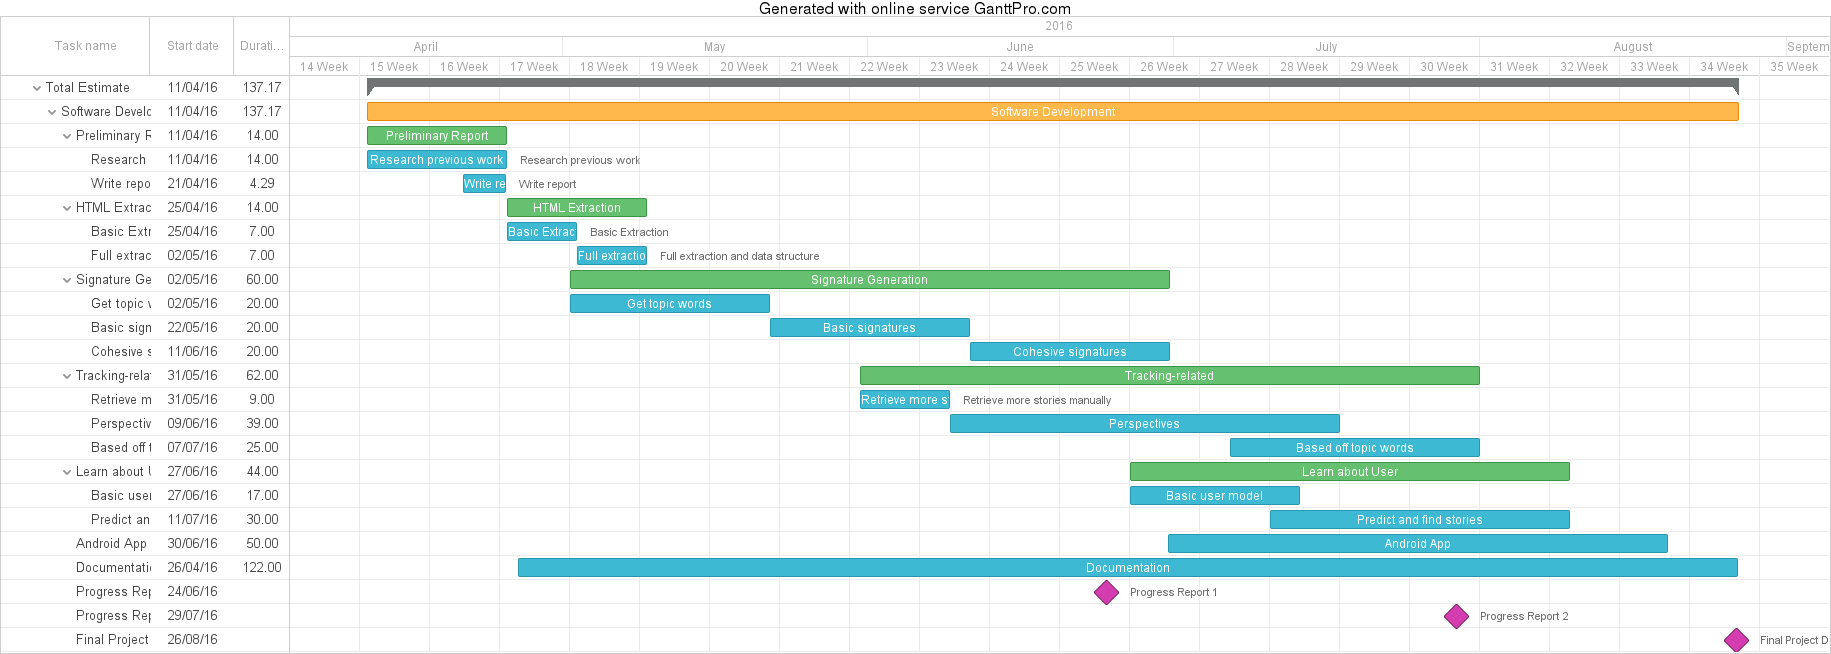
\includegraphics[scale=0.45, angle=90]{gantt}
\end{figure}

\bibliographystyle{plain}
\bibliography{literature}

\end{document}